\documentclass[tikz,border=5pt]{standalone}
\usepackage{ctex,amsmath}
\usetikzlibrary{arrows.meta,calc,angles,quotes}
\tikzset{>=Latex,cord/.style={blue!65!black,thick},rack/.style={orange!85!black,line width=1.4pt},
force/.style={blue!65!black,very thick,->},react/.style={red!65!black,very thick,->}}
\begin{document}
\begin{tikzpicture}[font=\small]
\foreach \x/\kind in {0/1,5.9/2,11.8/3}{
\begin{scope}[xshift=\x cm]
\coordinate(A)at(2.1,3.2);\coordinate(B)at(0,0);\coordinate(C)at(4.6,0);
\coordinate(D)at(1.28,0);\coordinate(O)at(1.79,1.99);
\ifnum\kind=1 \coordinate(O)at(2.05,1.35);\fi
\ifnum\kind=3
 \coordinate(A)at(2.3,3.983717);\coordinate(D)at(1.232566,0);
 \coordinate(O)at(1.605094,1.390291);
\fi
\draw[thick](A)--(B)--(C)--cycle;
\ifnum\kind>1 \draw[rack](A)--(D);\fi
\draw[cord](O)--(A);\draw[cord](O)--(B);\draw[cord](O)--(C);
\fill(O)circle[radius=.035cm]node[above right,xshift=1pt]{$O$};
\node[above]at(A){$A$};\node[below left]at(B){$B$};\node[below right]at(C){$C$};
\ifnum\kind>1 \node[below]at(D){$D$};\fi
\ifnum\kind=3
 \pic[draw,angle radius=.8cm,angle eccentricity=2.5,"$15^\circ$"]{angle=B--A--D};
 \node[below]at(2.3,-.65){$AB=BC=CA$};
\else
 \ifnum\kind=1\node[below]at(2.3,-.65){点 $O$ 可在三角形内移动};
 \else\node[below]at(2.3,-.65){点 $O$ 限于线段 $AD$};\fi
\fi
\end{scope}}
\end{tikzpicture}
\begin{tikzpicture}[font=\small]
\coordinate(A)at(2.326,1.485);\coordinate(B)at(0,0);\coordinate(C)at(3.3,0);
\coordinate(O)at(1.804,.44);
\filldraw[fill=gray!9,thick](-.4,0)--(3.6,0)--(4.816,1.76)--(.816,1.76)--cycle;
\draw[gray,dashed](A)--(2.326,0);
\draw[cord](2.326,0)--(2.326,-1.18);
\draw[cord](B)--(0,-1.42);\draw[cord](C)--(3.3,-1.42);
\draw[cord](O)--(A);\draw[cord](O)--(B);\draw[cord](O)--(C);
\foreach \xx/\yy in {0/-1.62,2.326/-1.38,3.3/-1.62}{
 \filldraw[fill=gray!20](\xx-.16,\yy-.2)rectangle(\xx+.16,\yy+.2);
 \node at(\xx,\yy){$m$};}
\foreach \pt/\place in {A/left,B/below left,C/above right}{
 \filldraw[fill=white](\pt)circle[radius=.055cm];\node[\place]at(\pt){$\pt$};}
\fill(O)circle[radius=.045cm]node[above left]{$O$};
\draw[gray](2.39,1.54)--(2.75,2.15)--(3.6,2.15);
\node[right]at(3.6,2.15){光滑小孔};
\draw[gray,->](5.2,1.2)--(5.2,.4)node[right]{$\boldsymbol g$};
\node[below]at(2.2,-2.17){水平板上绳段与板下悬挂段；虚线表示被板遮住的绳段};
\end{tikzpicture}
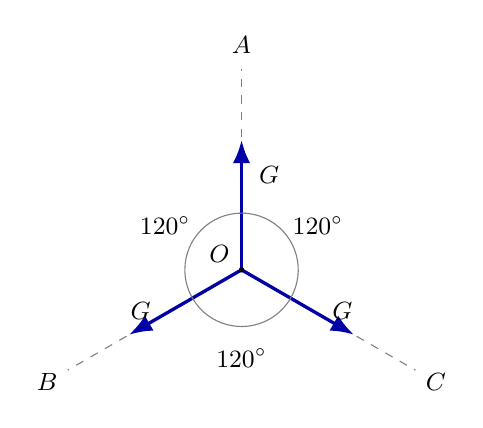
\begin{tikzpicture}[font=\small]
\coordinate(O)at(0,0);
\foreach \ang/\letter in {90/A,210/B,330/C}{
 \draw[gray,dashed](O)--(\ang:2.55);\node at(\ang:2.85){$\letter$};
 \draw[force](O)--(\ang:1.65);}
\node[right]at(.10,1.2){$G$};\node at(-1.28,-.52){$G$};\node at(1.28,-.52){$G$};
\draw[gray](90:.72)arc[start angle=90,end angle=210,radius=.72];
\draw[gray](210:.72)arc[start angle=210,end angle=330,radius=.72];
\draw[gray](330:.72)arc[start angle=330,end angle=450,radius=.72];
\node at(150:1.12){$120^\circ$};\node at(270:1.12){$120^\circ$};\node at(30:1.12){$120^\circ$};
\fill(O)circle[radius=.035cm];\node at(-.28,.2){$O$};
\end{tikzpicture}
\begin{tikzpicture}[font=\small]
\coordinate(A)at(1.5,2.598);\coordinate(B)at(0,0);\coordinate(C)at(3,0);
\coordinate(O)at(1.5,.866);\coordinate(Os)at(1.5,-.866);\coordinate(Cs)at(1.5,-2.598);
\draw[thick](A)--(B)--(C)--cycle;
\draw[cord](O)--(B);\draw[cord](O)--(C);
\draw[orange!85!black,thick](B)--(Os)--(Cs)--cycle;
\draw[gray,dashed](B)--(Os);
\draw[red!65!black,line width=1.35pt](A)--(Cs);
\node[above]at(A){$A$};\node[left]at(B){$B$};\node[right]at(C){$C$};
\node[right]at(O){$O$};\node[right]at(Os){$O^*$};\node[below]at(Cs){$C^*$};
\node[right,align=left]at(3.4,1.4){绕 $B$ 顺时针转 $60^\circ$\\$O\mapsto O^*,\ C\mapsto C^*$};
\node[right,align=left]at(3.4,-1.35){$OO^*=BO$\\$O^*C^*=OC$};
\draw[gray,->](3.36,-1.3)--(1.59,-1.45);
\draw[gray,->](.58,.34)arc[start angle=30,end angle=-30,radius=.67];
\end{tikzpicture}
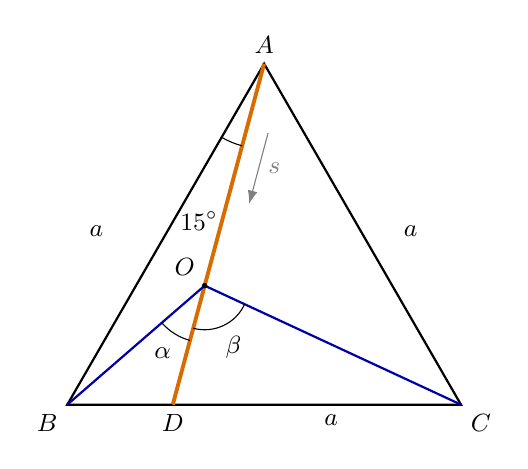
\begin{tikzpicture}[font=\small]
\coordinate(A)at(2.5,4.330127);\coordinate(B)at(0,0);\coordinate(C)at(5,0);
\coordinate(D)at(1.339746,0);\coordinate(O)at(1.744667,1.511186);
\draw[thick](A)--(B)--(C)--cycle;
\draw[rack](A)--(D);\draw[cord](B)--(O)--(C);
\pic[draw,angle radius=1.08cm,angle eccentricity=2.0,"$15^\circ$"]{angle=B--A--D};
\pic[draw,angle radius=.72cm,angle eccentricity=1.4,"$\alpha$"]{angle=B--O--D};
\pic[draw,angle radius=.56cm,angle eccentricity=1.55,"$\beta$"]{angle=D--O--C};
\node[above]at(A){$A$};\node[below left]at(B){$B$};\node[below right]at(C){$C$};\node[below]at(D){$D$};
\fill(O)circle[radius=.035cm]node[above left]{$O$};
\node[left]at(.58,2.2){$a$};\node[right]at(4.15,2.2){$a$};\node[below]at(3.35,0){$a$};
\draw[gray,->](2.55,3.45)--(2.31,2.55)node[midway,right]{$s$};
\end{tikzpicture}
\begin{tikzpicture}[font=\small]
\coordinate(O)at(0,0);\coordinate(A)at(.569,2.125);\coordinate(D)at(-.569,-2.125);
\coordinate(B)at(-1.663,-1.44);\coordinate(C)at(1.995,-.926);
\draw[rack](A)--(D);
\draw[gray,dashed](O)--(B)node[left]{$B$};\draw[gray,dashed](O)--(C)node[right]{$C$};
\node[above]at(A){$A$};\node[below]at(D){$D$};
\draw[force](O)--(.44,1.642)node[above right]{$G$};
\draw[force](O)--(-1.284,-1.112)node[left]{$G$};
\draw[force](O)--(1.542,-.716)node[right]{$G$};
\draw[react](O)--(-.966,.259)node[above left]{$\boldsymbol R$};
\pic[draw,angle radius=.66cm,angle eccentricity=1.4,"$\alpha$"]{angle=B--O--D};
\pic[draw,angle radius=.47cm,angle eccentricity=1.55,"$\beta$"]{angle=D--O--C};
\draw[gray,->](1.16,-1.46)--(.927,-2.33)node[right]{$\boldsymbol u$};
\draw[gray,->](1.16,-1.46)--(2.03,-1.693)node[right]{$\boldsymbol n$};
\fill(O)circle[radius=.035cm]node[above left]{$O$};
\node[below]at(0,-2.9){无摩擦支架反力垂直于 $AD$};
\end{tikzpicture}
\end{document}
